%start preamble
\documentclass[paper=a4,fontsize=11pt]{scrartcl}%kind of doc, font size, paper size

\usepackage{fontspec}
\defaultfontfeatures{Ligatures=TeX}
%\setsansfont{Liberation Sans}
\usepackage{polyglossia}	
\setdefaultlanguage[spelling=new, babelshorthands=true]{german}
			
\usepackage{amsmath}%get math done
\usepackage{amsthm}%get theorems and proofs done
\usepackage{graphicx}%get pictures & graphics done
\graphicspath{{pictures/}}%folder to stash all kind of pictures etc
\usepackage{amssymb}%symbolics for math
\usepackage{amsfonts}%extra fonts
\usepackage{caption}%captions under everything
\usepackage{listings}
\numberwithin{equation}{section} 
\usepackage{float}%for garphics and how to let them floating around in the doc
\usepackage{xcolor}%nicer colors, here used for links
\usepackage{dsfont}
\usepackage{stmaryrd}
\usepackage{geometry}
\usepackage{hyperref}
\usepackage{fancyhdr}
\usepackage{multicol}
\usepackage{csquotes}
\usepackage{enumitem}

\usepackage{tikz}
\usetikzlibrary{arrows}

\usepackage[backend=biber,style=alphabetic,
citestyle=alphabetic]{biblatex} %biblatex mit biber laden
\addbibresource{sources.bib}

%settings colors for links
\hypersetup{
    colorlinks,
    linkcolor={blue!50!black},
    citecolor={blue},
    urlcolor={blue!80!black}
}

\definecolor{pblue}{rgb}{0.13,0.13,1}
\definecolor{pgreen}{rgb}{0,0.5,0}
\definecolor{pred}{rgb}{0.9,0,0}
\definecolor{pgrey}{rgb}{0.46,0.45,0.48}


\pagestyle{fancy}
\lhead{Netzwerke und verteilte Systeme\\
 Übung SoSe 2022}
\rhead{Informatik in Kultur und Gesundheit\\HTW-Berlin FB 4}
\lfoot{IP Routing}
\cfoot{}
\fancyfoot[R]{\thepage}
\renewcommand{\headrulewidth}{0.4pt}
\renewcommand{\footrulewidth}{0.4pt}

\lstdefinestyle{Bash}{
  language=bash,
  showstringspaces=false,
  basicstyle=\small\sffamily,
  numbers=left,
  numberstyle=\tiny,
  numbersep=5pt,
  frame=trlb,
  columns=fullflexible,
  backgroundcolor=\color{gray!20},
  linewidth=0.9\linewidth,
  %xleftmargin=0.5\linewidth
}


%%here begins the actual document%%
\newcommand{\horrule}[1]{\rule{\linewidth}{#1}} % Create horizontal rule command with 1 argument of height


\begin{document}
\begin{center}
\Large{\textbf{Übungsblatt 4 -- Routing, ICMP, IP \& ARP}}
\end{center}

\begin{center}\Large{\textbf{Aufgabe A -- Routing-Algorithmen}}\end{center}\vskip0.25in
\begin{enumerate}
	\item In der Vorlesung haben sie zwei Routing-Algorithmen kennen gelernt. Dies sind das Distanz-Vektor- und Link-State-Routing. Beide ermöglichen es den kürzesten Weg durch einen Graphen zu finden (Shortest-Path-Problem).\\
	Für gewöhnlich wird für das Distanz-Vektor-Routing der Bellman-Ford-Algorithmus verwandt, das Link-State-Routing nutzt den Dijkstra-Algorithmus. \cite[S. 363ff]{Kurose2012}
	\begin{enumerate}
		\item Erläutern sie das Link-State-Routing unter Nutzung des Dijkstra-Algorithmus \cite[S. 366]{Kurose2012}.
		\item Erläutern sie das Distanz-Vektor-Routing unter Nutzung des Bellman-Ford-Algorithmus \cite[S. 371]{Kurose2012}.
		\item In welchen Protokollen finden diese beiden Protokollen Verwendung? Ist diesen Protokollen etwas gemein?
		\item Erläutern sie die fundamentalen Unterschiede beider Lösungsansätze. Was unterscheidet Bellman-Ford und Dijkstra? \textbf{Hinweis:} Wie betrachtet der Algorithmus den Graph?
		\item Das Exterior-Gateway-Protokoll nutzt keines der beiden obigen Algorithmen, sondern ein Pfad-Vektor-Protokoll. Können sie Gründe nennen, warum weder Bellman-Ford noch Dijkstra genutzt wird?
		\item Diskutieren sie, ob der Bellman-Ford-Algorithmus für das Link-State-Routing und der Dijkstra-Algorithmus für das Distanz-Vektor-Routing genutzt werden könnte.
	\end{enumerate}
	\item Gegeben sei folgender Graph:
	\begin{center}
	\begin{tikzpicture}[->,>=stealth',shorten >=1pt,auto,node distance=3cm,
                    thick,main node/.style={circle,draw,font=\sffamily\Large\bfseries}]

  \node[main node] (A) {A};
  \node[main node] (B) [below right of=A] {B};
  \node[main node] (C) [above right of=A] {C};
  \node[main node] (D) [right of=B] {D};
  \node[main node] (E) [above of=D] {E};
  \node[main node] (F) [right of=E] {F};

  \path[every node/.style={font=\sffamily\small}]
    	(A) edge node [left] {10} (B)
	    (A) edge node [left] {20} (C)
	    (C) edge node [left] {33} (E)
	    (C) edge node [left] {20} (D)
	    (B) edge node [left] {10} (E)
	    (D) edge node [left] {20} (E)
	    (D) edge node [left] {2} (F)
	    (E) edge node [left] {1} (F)
    ;
	\end{tikzpicture}
	\end{center}
	Finden sie den kürzesten Weg vom Knoten $A$ zum Knoten $F$!
	\begin{enumerate}
		\item Nutzen sie zunächst den Dijkstra-Algorithmus.
		\item Nutzen sie den Bellman-Ford-Algorithmus.
	\end{enumerate}
	\item Das \emph{Border Gateway Protocol} wendet den sogenannte \enquote{Best Path Algorithm} an. Erläutern sie wie ein BGP Router die Route wählt, falls mehrere Pfade (Path/Teilrouten) verfügbar sind. \footnote{In der echten Welt ist dies durchaus komplexer, s. \url{https://www.ietf.org/rfc/rfc4271.txt.}}
	\item Im gewöhnlichen BGP-Routing werden die Policies als \enquote{Valley Free} bezeichnet. Erläutern sie warum \enquote{Valley Free Routing} eine gute Policy-Entscheidung ist.\footnote{Dieser Blog-Eintrag könnte hilfreich sein: \url{https://blog.ipspace.net/2018/09/valley-free-routing.html}}
\end{enumerate}

\begin{center}\Large{\textbf{Aufgabe B -- Traceroute}}\end{center}\vskip0.2in
\begin{enumerate}
	\item Lesen sie die folgenden Artikel:\\
	\url{https://www.freebsd.org/cgi/man.cgi?query=traceroute}\\
	\url{https://docs.freebsd.org/de_DE.ISO8859-1/books/handbook/network-routing.html} Abschnitt 31.2.3. Problembehandlung
	Beantworten sie anschließend folgende Fragen:
	\begin{enumerate}
		\item Wofür wird Traceroute genutzt?
		\item Wie wird Traceroute umgesetzt, d.h. wie läuft eine Routen-Verfolgung ab? 
		\item Welche ICMP-Messages werden für die Realisierung genutzt?
		\item Welche Limitationen ergeben sich aus dieser Umsetzung?
		\item Dokumentieren sie die Syntax, sowie die Bedeutung von Traceroute beispielhaft.
	\end{enumerate}
\end{enumerate}	

\begin{center}\Large{\textbf{Aufgabe C -- Address Resolution Protocol (ARP) \& Neighbor Discovery Protocol (NDP)}}\end{center}\vskip0.25in
Es sollte ihnen aufgefallen sein, dass in der zweiten Übung (Geswitchte Netze) ihr Netzwerk in der Planung zwar IP-Adressen nutzt, aber kein Router Verwendung fand. Im Labor würde ein Switch zum Einsatz kommen. Switches sind OSI-Layer 2 Geräte und kommen ohne IP-Adressen zurecht. Ihre VMs verlangen jedoch zwingend eine IP-Adresse von Ihnen.
\begin{enumerate}
		\item Recherchieren sie mithilfe der Literatur was \emph{ARP} ist \cite[Kap. 5.4f]{Kurose2012}
		\item Wie adressiert ein Switch die Frames zwischen den Endknoten (also den VMs)? \textbf{Hinweis:} Wie oben bereits erwähnt geschieht dies nicht mittels IP-Adressen.
		\item Erläutern sie das \emph{MAC}-Adressschema. Kann dieses Adressschema auch zu Problemen führen?
		\item Unter \emph{IPv6} gibt es kein \emph{ARP}, wie wird dies dort gehandhabt? Bzw. wie funktioniert \emph{NDP}?
		\item Recherchieren sie wozu die Werkzeuge \emph{arp} und \emph{ip neigh} in unixoiden Betriebssystemen genutzt werden können.
		\item Recherchieren sie die grundlegende Syntax und Semantik von \emph{arp} sowie \emph{ip neigh}.
\end{enumerate}


\begin{center}\Large{\textbf{Aufgabe D -- IP}}\end{center}\vskip0.2in
Im Moodle-Kurs liegt eine Zip-Datei \path{network_packets.zip}. Diese enthält verschiedene Dateien die sie auf verschiedene Arten in Wireshark öffnen können. Sie sollen diese Pakete analysieren. Teilweise sind in diesen Paketen Passwörter und Zugangsdaten zu finden, in einigen Fällen können ganze Nachrichten oder Geräteinformationen gefunden werden.

\begin{enumerate}
	\item Öffnen sie aus dem Zip-Archiv die Datei \path{ch1.pcap} mit Wireshark. Stellen sie den Filter auf \emph{IP}. Suchen sie sich ein IP-Paket heraus. Wo finden sie folgenden Informationen?
	\begin{itemize}
		\item Welche Adressen sind im Paket enthalten? Wie viele sind dies?
		\item Ethernet hat eine Prüfsumme, TCP ebenfalls. Hat IP eine Prüfsumme?
		\item Ist IP ein verbindungsorientiertes Protokoll? Begründen sie ihre Antwort anhand der eben vorgenommen Analyse. Welche Information des Pakets legt ihren Schluss dar.
		\item Ein IP-Paket besteht aus Header und Payload. Wo und wie wird die Trennung festgelegt?
		\item Wo ist die Information der nächst höheren Protokollebene zu finden?
	\end{itemize}
\end{enumerate}

\begin{center}\Large{\textbf{Aufgabe E -- ICMP}}\end{center}\vskip0.2in
Da die Befehle \emph{ping} und \emph{traceroute} \emph{ICMP} nutzen, sollen Sie mit Wireshark solche Request mitverfolgen.
\begin{enumerate}
	\item Setzen sie alle notwendigen Parameter um Wireshark mitlaufen zu lassen, sodass sie die ICMP-Nachrichten mitverfolgen können.
	\item Nutzen sie Traceroute um einen Rechner mit seinen DNS-Namen zu erreichen (bspw.: \url{mi.fu-berlin.de}).
	\item Ping auf die IP-Adresse ihres Routers. \\\textbf{Hinweis:} Sie können diese durch \emph{netstat} in Erfahrung bringen. 
	\begin{lstlisting}[style=Bash, language=Bash]
#or.
netstat -nr
Kernel IP routing table
Destination     Gateway         Genmask         Flags   MSS Window  irtt Iface
0.0.0.0         XXX.XXX.XXX.1   0.0.0.0         UG        0 0          0 pf-bridge
XXX.XXX.128.0   0.0.0.0         255.255.255.0   U         0 0          0 igb0
XXX.XXX.0.0     0.0.0.0         255.255.255.128 U         0 0          0 igb1
...
XXX.XXX.32.128  0.0.0.0         255.255.255.248 U         0 0          0 igb3
...
	\end{lstlisting}
	\item Nehmen sie nun eine ihrer Ping-Anfragen und analysieren sie diese mithilfe Wiresharks genauer.
	\begin{enumerate}
		\item Auf welcher Ebene des OSI-Modells ist das ICMP-Protokoll einzuordnen? Begründen sie ihre Antwort!
		\item Analysieren sie mithilfe Wiresharks den Aufbau eines ICMP-Pakets. Wie ist der generische Aufbau? Skizzieren sie den Aufbau mithilfe der in Abb. \ref{icmp1}.
		\begin{figure}[H]
		\centering
		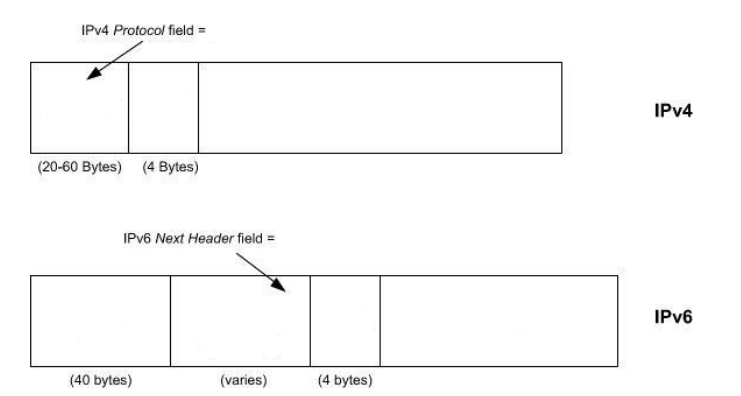
\includegraphics[scale=0.5]{icmp1}
		\caption{Generischer Aufbau eines ICMP-Pakets für IPv4 und IPv6.}
		\label{icmp1}
		\end{figure}
		\item Welche Nachrichtentypen werden für den Ping-Messages genutzt? Wo sind die Nachrichtentypen zu finden?
		\item Skizzieren sie mithilfe von Abb.\ref{icmp2} die ICMP-Nachricht und welche Informationen Wireshark ihnen liefert.
		\begin{figure}[H]
		\centering
		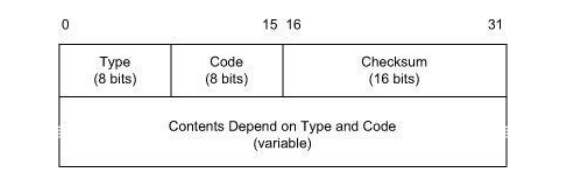
\includegraphics[scale=0.5]{icmp2}
		\caption{Nutzlast eines ICMP-Pakets.}
		\label{icmp2}
		\end{figure}
	\end{enumerate}
	\item Starten sie eine Routen-Verfolgung via \emph{traceroute} auf eine beliebige Adresse. Verfolgen sie dabei die Ausgabe auf der Konsole und Wireshark (Filtern sie in Wireshark entsprechend). Spiegeln sich die Einträge in Wireshark mit denen auf der Kommandozeile?
	\item Welche ICMP-Nachrichten wurden hier verwendet?
	\item Erläutern sie die genaue Routen-Verfolgung mithilfe der ICMP-Nachrichten. Welches Feld wird hier genutzt um jeden Hop \enquote{verfolgen} zu können?
	\item Überlegen sie sich zunächst anhand Ihrer Recherche was \emph{traceroute} in etwa ausgeben müsste, wenn sie auf der VM eine Route von einem Rechner $A$ zu einem Rechner $B$ verfolgen würden. Wobei beide Rechner zu unterschiedlichen LANs gehören. 
	\item Nutzen Sie anschließend \emph{traceroute} um sich die Router zwischen zwei VMs anzeigen zu lassen. Stimmen Ihre theoretische Überlegungen mit denen von \emph{traceroute} überein? Falls nicht, sollten Sie analysieren woran dies liegen könnte.
\end{enumerate}

\begin{center}
\Large{\textbf{Aufgabe F - Bestimmung des physischen Rechners zu einer IP-Adresse -- ARP}}
\end{center}\vskip0.25in
Sie haben bereits theoretisch recherchiert, wie die Zuordnung von physischer Adresse zu einer IP-Adresse vonstatten geht. Im Folgenden sollen sie herausfinden, ob die Auflösung von IP-Adresse auf physische Adresse wirklich analog zu ihren theoretischen Recherchen abläuft.
\begin{enumerate}
	\item Um einen ARP-Request auszulösen können sie das Werkzeug \emph{arp} nutzen. Lesen sie in der \emph{man}-Page:
	\begin{itemize}
		\item Wie können sie sich ihre MAC-Adresse und Interface anzeigen lassen?
		\item Wie können sie sich den ARP-Table ausgeben lassen?
		\item Wie leeren sie den ARP-Cache?
	\end{itemize}
	\item Finden sie mithilfe Wiresharks heraus, wie die Adressauflösung funktioniert.
		\begin{enumerate}
			\item Starten sie Wireshark und stellen sie das korrekte Interface ein.
			\item Leeren sie zunächst den ARP-Cache.
			\item Pingen sie nun einen Rechner an, den sie vorhin noch nicht \enquote{angepingt} haben. Die dafür ausgetauschten Pakete werden nun \enquote{gesnifft}.
			\item Beenden sie das Mitschneiden des Netzwerksverkehrs und setzen sie als Filtern die MAC-Adresse ihres Adapters.
			\item Versuchen sie über den Mitschnitt herauszufinden, wie die Bestimmung des zugehörigen Netzadapters und die MAC-Adresse erfolgt.
		\end{enumerate}
	\item Damit ihr Rechner nicht jedes mal eine Auflösung veranlassen muss, werden die ARP-Informationen lokal in einem Cache zwischengespeichert (\enquote{cached}).
\begin{enumerate}
	\item Lassen sie sich Ihren aktuellen ARP-Cache anzeigen. Welche Informationen können sie diesem entnehmen?
	\item Schauen sie kurz nach, wie lange der ARP-Cache Einträge vorhält.
	\item Lassen sie zwei VMs die IP-Adressen tauschen. Dies sollte möglichst schnell umgesetzt werden!
	\item Versuchen sie nun durch eine dritte VM eine \enquote{alte} IP-Adresse zu erreichen. Werden die Daten an den richtigen Knoten übermittelt?
	\item Verfolgen sie die Datenübermittlung per Wireshark mit.
\end{enumerate}
\end{enumerate}

\printbibliography

\end{document}
